\documentclass{article}
\usepackage[x11names, svgnames, rgb]{xcolor}
\usepackage[utf8]{inputenc}
\usepackage{tikz}
\usetikzlibrary{snakes,arrows,shapes}
\usepackage{amsmath}
%
%

%

%

\begin{document}
\pagestyle{empty}
%
%
%

\enlargethispage{100cm}
% Start of code
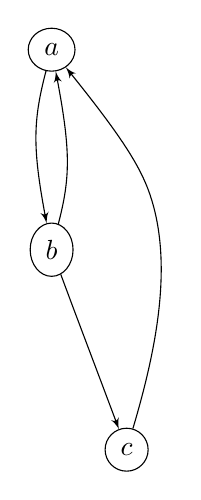
\begin{tikzpicture}[>=latex',line join=bevel,]
%%
\node (a) at (27.0bp,162.0bp) [draw,ellipse] {$a$};
  \node (b) at (27.0bp,90.0bp) [draw,ellipse] {$b$};
  \node (c) at (54.0bp,18.0bp) [draw,ellipse] {$c$};
  \draw [->] (a) ..controls (20.297bp,136.51bp) and (20.048bp,126.85bp)  .. (b);
  \draw [->] (b) ..controls (33.714bp,115.83bp) and (33.948bp,125.37bp)  .. (a);
  \draw [->] (b) ..controls (36.514bp,64.335bp) and (40.334bp,54.431bp)  .. (c);
  \draw [->] (c) ..controls (64.687bp,53.977bp) and (70.486bp,83.656bp)  .. (63.0bp,108.0bp) .. controls (59.714bp,118.69bp) and (53.46bp,129.15bp)  .. (a);
%
\end{tikzpicture}
% End of code

%
\end{document}
%



